\documentclass[]{report}
\usepackage{graphicx}
\usepackage{amsmath}
\usepackage{amsfonts}
\usepackage{amssymb}

% Title Page
\title{Homework Set 1}
\author{Miles Van de Wetering
	\and
	Cierra Shawe
	\and
	Charles Dwayne}


\begin{document}
\maketitle

\section*{Problem 1}
Draw all possible DFS trees rooted at x for the following graph. Mark, tree, forward,
backward, and cross edges
\begin{center}
	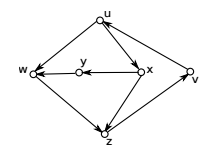
\includegraphics[]{hw1_p1_graph.png}
	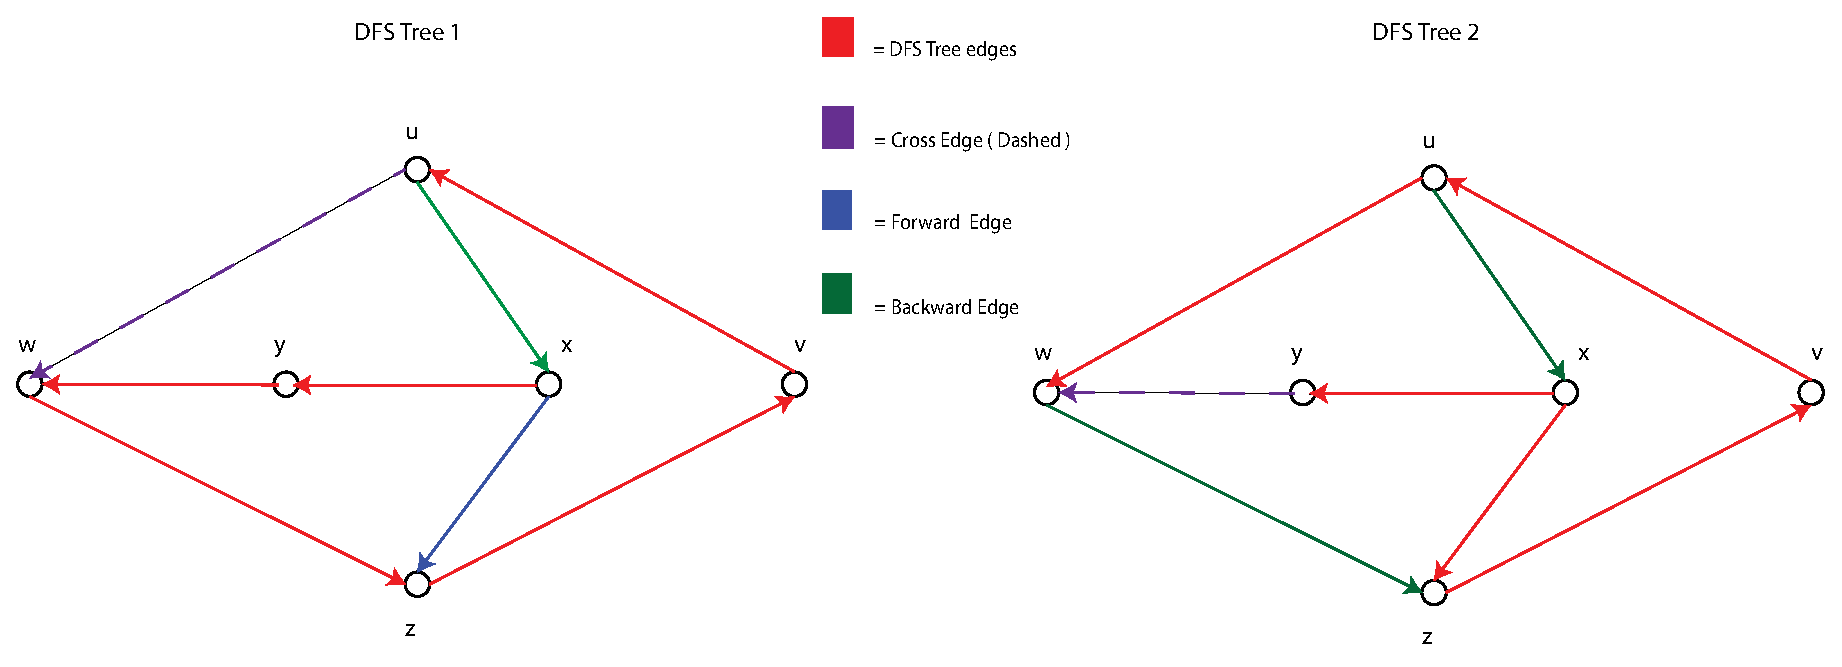
\includegraphics[]{cs420-hw2.eps}
\end{center}

\section*{Problem 3}
Let G = (V, E) be an undirected unweighted graph, and let s, t $\in$ V. Show that at least one of the following conditions hold:
\begin{enumerate}
	\item The distance between s and t is at most $\sqrt{V} + 1$.
	\item There is a subset S $\subset$ V of cardinality at most $\sqrt{V}$ whose removal disconnects s and t.
\end{enumerate}

In order to show this we will build an argument based on three truths:
\begin{enumerate}
	\item Any single path, in any graph, may be destroyed by removing a single vertex along that path.
	\item If (1) is false, then every path  between s and t must pass through at least $\sqrt{V} + 3$ vertices.
	\item The most vertices that we may need to remove in order to disconnect every path from s to t is the number of paths between s and t, assuming that these paths share no vertices except s and t. If they share more vertices, then we can remove fewer nodes and still succeed. (Menger Theorem)
\end{enumerate}
	\smallskip
	
	From these three premises, we may conclude that the maximum number of unique paths that can exist between s and t is less than or equal to the number of non start-end nodes available in the graph, divided by the number of non start-end nodes required to construct a unique path:  
	\bigskip
	
	$\frac{V -2}{\sqrt{V} + 1} \leq \frac{V}{\sqrt{V} + 1} \leq \frac{V}{\sqrt{V}} = \sqrt{V}$
	\bigskip

	Therefore, the number of unique paths that may exist is less than or equal to $\sqrt{V}$, and therefore the maximum number of nodes that we must remove in order to disconnect s and t, given (1), is strictly bounded by $\sqrt{V}$, thus (2) holds.
	\bigskip
	
	Since $\neg(1)$ implies (2), $\neg(2)$ must imply (1).

\end{document}          
